\documentclass[a4paper,12pt]{article}
\usepackage{cmap}
\usepackage[cp1251]{inputenc}
\usepackage[english, ukrainian, russian]{babel}
\usepackage[left=2cm,right=1.5cm,top=1cm,bottom=1cm]{geometry}
\usepackage{amssymb}
\usepackage{graphicx}
\usepackage{tabularx}
\usepackage{slashbox}

\begin{document}

\pagenumbering{gobble}


\begin{large}

\begin{center}
\section*{Application of natural language processing and fuzzy logic to disinformation detection.}
\end{center}

\medskip

\begin{center}
\textbf{Abstract}
\end{center}

Natural language processing (NLP) is a field of computer science that is concerned with processing, collection and analysis of data encoded in natural language, such as speech, written text, online posts, etc.
In this article we use some of the well known NLP techniques to analyse online data for possible disinformation, combining them, and we apply fuzzy logic rules to analyse the results for possible false-positives.



\medskip
\medskip

\hrule height 1pt
\vskip 3pt \hrule

\medskip
\medskip


\section*{Introduction.}

In today's interconnected world, the rapid spread of information across digital platforms has amplified the challenge of combating disinformation. False and misleading information can have far-reaching consequences, from swaying public opinion to impacting political and social stability. Effective detection of disinformation is crucial, and advanced computational techniques offer promising solutions. This article explores the application of Natural Language Processing (NLP) techniques for detecting disinformation and leverages fuzzy logic to refine these methods, reducing the incidence of false positives.

Natural Language Processing (NLP) encompasses a range of computational techniques aimed at understanding and processing human language. For disinformation detection, several NLP methods are particularly effective. TF-IDF (Term Frequency-Inverse Document Frequency) measures the importance of a word in a document relative to a collection of documents (corpus). This statistical measure helps highlight terms that are particularly significant in identifying unique content, which is crucial in spotting disinformation. N-grams, on the other hand, capture contiguous sequences of words, providing a more comprehensive understanding of context and word associations. These methods, when combined, offer a robust framework for analyzing textual data and identifying patterns indicative of disinformation.

While NLP techniques are powerful, they can sometimes produce false positives, mistakenly classifying truthful information as disinformation. This is a significant challenge, as over-correcting for disinformation can undermine the credibility of legitimate content. To address this, we integrate fuzzy logic into the disinformation detection process. Fuzzy logic, with its ability to handle uncertainty and partial truths, provides a means to refine NLP-based disinformation detection, ensuring a more accurate and reliable outcome.

Fuzzy logic allows for degrees of truth, making it well-suited to handle the nuances and ambiguities inherent in natural language. By applying fuzzy logic, we can assess the likelihood of a piece of information being disinformation rather than making a binary decision. This probabilistic approach helps to capture the subtleties that NLP techniques might miss, reducing the chances of misclassifying truthful information. By incorporating features such as the credibility of sources, historical accuracy of the content, and the overall sentiment, fuzzy logic systems can better differentiate between disinformation and legitimate information.


\section*{Overview of linguistic analysis methods.}

Most tasks related to text processing in data science can be accomplished with relatively simple methods that we can easily understand without any reference to sophisticated machine learning: methods such as TF-IDF vectors and N-gram language models.

TF-IDF vectors: This method also uses a vector representation of the text, but takes into account not only the frequency of words in the document, but also their information content. TF-IDF (the term frequency inverse of document frequency) determines how well a document matches the analysis criteria with other documents in the collection. This allows us to identify keywords or terms that may indicate disinformation.

N-gram language models: This method is used to analyze text based on sequences of fixed length words (n-grams). The difference from the bag-of-words model is that it takes into account word order. This can be useful for identifying phrases or language structures that are often found in disinformation materials.

We can represent documents using a frequency matrix and an $m\times n$ matrix, where $m$ denotes the number of documents and $n$ denotes the size of the dictionary (i.e., the number of unique words in all documents).

\begin{center}
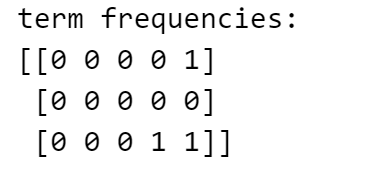
\includegraphics[scale=0.8]{nlp5.png}
\end{center}

Now let's build a matrix that contains the number of words (frequency of occurrence) for all documents.

An obvious problem with using conventional term frequency counts to represent a document is that the document vector will often be 'dominated' by very common words, e.g: 'of', 'the', 'is'. This problem can be mitigated to some extent by excluding the so-called 'stop words' (common English words such as 'the', 'a', 'of' that are not considered relevant to specific documents) from the term frequency matrix. However, this ignores the case when a word that is not a common stop word still occurs in a very large number of documents. Intuitively, we expect that the most 'important' words in a document are those that appear in only a relatively small number of documents, so we want to discard the weight of very frequently used terms.



$$idf_{j}=\log(\frac{N_{documents}}{N_{documents\textmd{ }with\textmd{ }word\textmd{ }j}}).$$

For example, if a word appears in every document, the inverse frequency weight of the document will be zero ($\log(1)$). Conversely, if a word appears in only one document, its inverse frequency in the document will be $\log(N_{documents})$.

\begin{center}
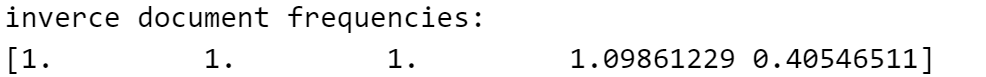
\includegraphics[scale=0.8]{nlp6.png}
\end{center}

The combination of 'term frequency inverse document frequency' (TF-IDF) simply scales the columns of the term frequency matrix by the inverse document frequency. This way, we still have an effective bag of words representing each document, but we do so with weights derived from the inverse document frequency: we discard words that occur very frequently and increase the weight of less frequent terms.

\begin{center}
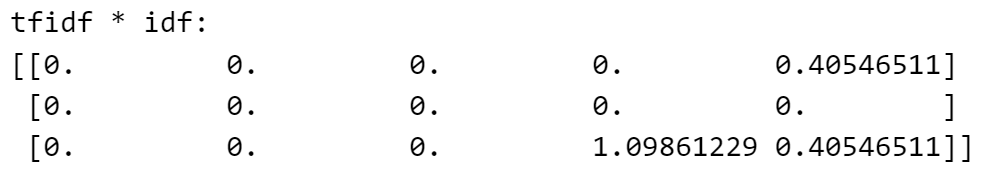
\includegraphics[scale=0.8]{nlp7.png}
\end{center}

Given a TF-IDF matrix, one of the most common issues to solve is to compute the similarity between multiple documents in the corpus. The most common metric for this is to calculate the cosine similarity between two different documents. This is simply the normalized inner product between the vectors describing each document:

$$CosineSimilarity(x,y)=\frac{x*y}{||x||_{2}\cdot ||y||_{2}}$$


Cosine similarity is a number between zero (meaning that two documents have no terms in common) and one (meaning that two documents have exactly the same term frequency or TF-IDF representation). In data analysis, cosine similarity is often used to determine the similarity between two non-zero sets of values defined in the inner product space. The cosine similarity is the cosine of the angle between vectors; that is, it is the scalar product of the vectors divided by the product of their lengths. It follows that cosine similarity does not depend on the magnitudes of the vectors, but only on their angle.

\begin{center}
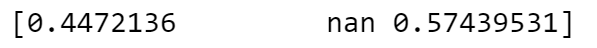
\includegraphics[scale=0.8]{nlp8.png}
\end{center}

We can calculate the cosine similarity between TF-IDF vectors in our corpus using the Euclidean product of two vectors.

N-gram analysis involves breaking down search queries into smaller fragments (n-grams) of 'n' words or terms. This helps to identify patterns or trends that might otherwise go unnoticed. In the context of our tool and most text analysis programs, n-grams refer to sequences of words.
Here is their distribution:

Unigram (1-gram): One word. For example, in the sentence 'I love ice cream', the unigrams are 'I', 'love', 'ice', and 'cream'.

Bigram (2-gram): A sequence of two adjacent words. In this sentence, the bigrams are 'I love', 'love ice', and 'ice cream'.

Trigram (3-gram): A sequence of three adjacent words. In this case, the trigrams are 'I love ice' and 'love ice cream'.

4-gram: A sequence of four adjacent words. If our sentence was 'I love ice cream', the 4-gram would be 'I love ice cream'.

N-grams are crucial in a variety of applications, including:

Text analysis: They help to understand the context and semantics of a text.

Machine learning and natural language processing: N-grams are used for predictive text input, speech recognition, and machine translation.

Search engines: Help improve search accuracy by considering word sequences rather than individual terms.

Understanding n-grams can offer a deeper understanding of text structure and patterns, making them invaluable for linguistic and computational analysis.

In this article we combine tf-idf analysis and n-gram text processing to achieve better detectability of texts containing disinformation.

\section*{Results of tf-idf and n-gram analysis.}

TF-IDF analysis is the main method in textual linguistics that assigns a numerical value to each word in a text, reflecting its importance in the relevant context. Using the TF-IDF method allows you to identify keywords and topics in texts, as well as determine their similarity to each other.

N-grams are sequences of n words in a text that allow you to analyze not only individual words but also their combinations. The use of n-grams improves the quality of analysis by providing more accurate detection of key terms and phrases in texts, as well as taking into account contextual information. The use of n-grams allows for a more detailed analysis of the text, which improves the analysis results and makes it more informative for further use.

On the other hand, as the size of n-grams increases, the similarity coefficients between texts decrease. This may be due to the fact that larger n-grams include more unique word sequences, which reduces the overall similarity between texts. In addition, large n-grams may be less effective in detecting similarities between texts with different topics and structures.

In our research, we first used simple TF-IDF analysis to example texts. The difference in cosine coefficients was not detectable at first:

\begin{center}
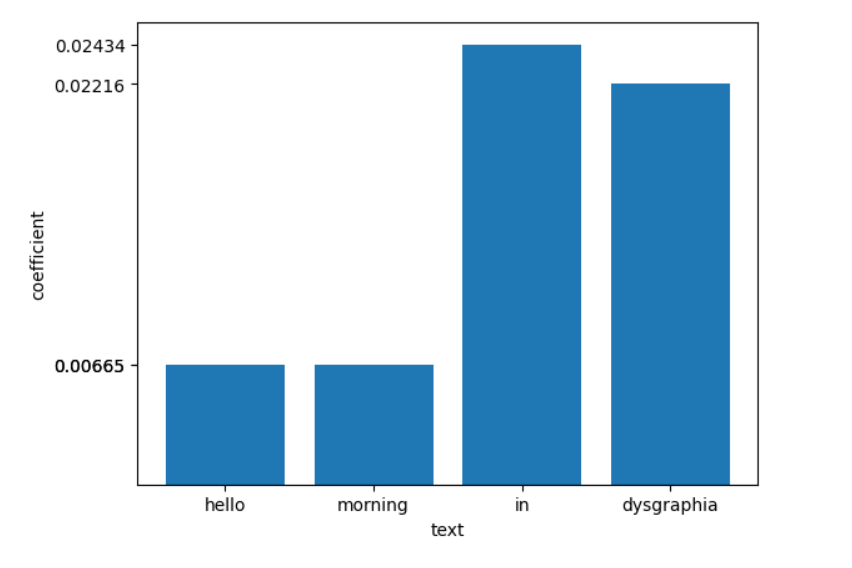
\includegraphics[scale=0.8]{nlp1.png}
\end{center}

After applying n-gram approach, we can see a more confident detection for disinformation texts. On the diagram below is the result of tf-idf approach combined with 3-gram processing of text.

\begin{center}
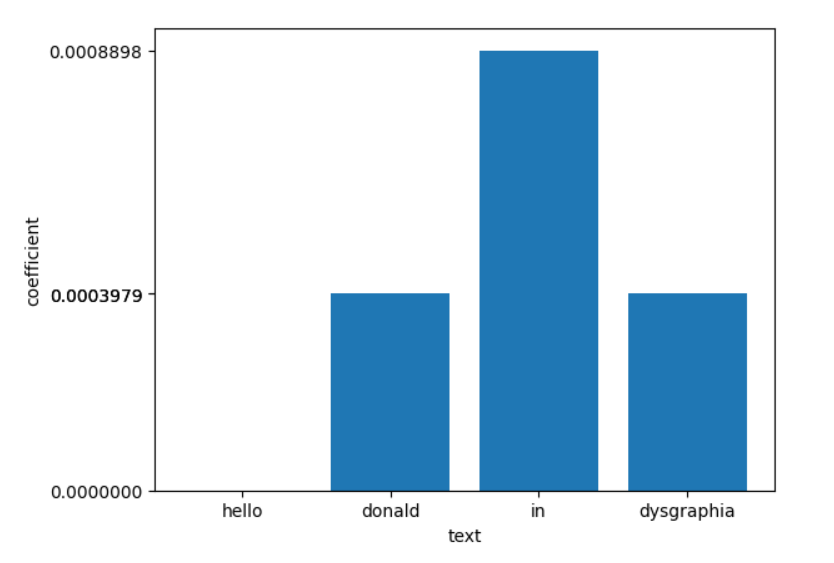
\includegraphics[scale=0.8]{nlp2.png}
\end{center}

As the length of n-grams increases, the number of times a particular n-gram can be seen to also decrease. This can lead to sparse data and make text modeling more difficult. The choice of n-gram size in text mining is a trade-off between sparsity and generalisability of the model, and should be made based on the specific task and data characteristics.


\section*{Fuzzy logic application.}

We can use fuzzy logic rules to detect possible false-positives in tf-idf and N-gram text analysis. Namely, we use another dataset with data samples, that can be misinterpreted as disinformation, but which are not actual examples of disinformation.

The result of tf-idf and N-gram analysis of text for disinformation we denote $c_{disinfo}$, and result of text analysis for false-positives we denote $c_{false-positive}$. Then, we have to setup the fuzzy rules for determining the resulting coefficient $c$. For example, if $c_{disinfo}$ is high and $c_{false-positive}$ is low, we determine, that the text is very likely a disinformation, and thus $c$ should be high. On the other hand, if $c_{disinfo}$ is high but $c_{false-positive}$ is also high, we can not conclusively say wether the text contains disinformation, and thus $c$ should have middle values. All these rules can be displayed in the table below:



Lets set up rules:


\begin{table}[h!]
\centering
\begin{tabular}{| p{4.6cm} || p{2cm} | p{2cm} | p{2cm} |}
    \hline
    \backslashbox{$c_{false-positive}$}{$c_{disinfo}$ } & \textbf{low} & \textbf{middle} & \textbf{high}  \\
    \hline
    \hline
    \textbf{low}  & neutral  & high & very high \\
    \hline
    \textbf{middle}  & low  & neutral & high \\
    \hline
    \textbf{high}  & very low  & low & neutral \\
    \hline
\end{tabular}
\end{table}

By applying the the fuzzy rules to our text example, we received a more confident detection.
We also used Gaussian membership functions, as we do not require much calculation for two parameters $c_{false-positive}$ and $c_{disinfo}$, and these membership functions provide more smoothness and concise notation as well as being nonzero at all points. Also, this type of membership function more accurately models many natural and real-world phenomena that exhibit gradual changes rather than abrupt transitions. This makes it particularly suitable for application in our research.


\begin{center}
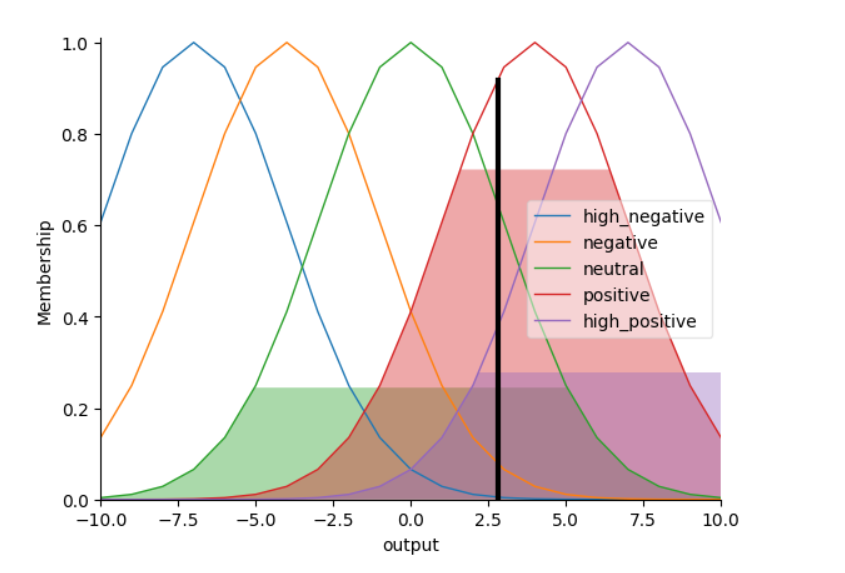
\includegraphics[scale=0.7]{nlp4.png}
\end{center}




\section*{Conclusion.}

This research has demonstrated, that the classical NLP approaches to text analysis, such as TF-IDf analysis combined with n-gram processing allows for pretty confident detection of disinformation.  The use of n-grams allows you to analyze the text more fully and thoroughly, which improves the analysis results and makes it more informative for further use. 


That detection can also be combined with cross-reference of the same text examples for false-positives. The results for cross-reference can be combined using fuzzy logic rules and Gaussian membership functions, giving a more confident detection of disinformation. Fuzzy logic has advantage over boolean logic in that case, since it allows to handle uncertainties in the detection. Its ability to handle uncertainty, imprecision, and gradual transitions makes it particularly useful where binary true-false decisions are insufficient.



\section*{References.}

1. Practical Natural Language Processing / S. Vajjala et al. O'Reilly Media, Inc., 2020.( https://www.oreilly.com/library/view/practical-natural-language/9781492054047/ )

2. Bressert E. SciPy and Numpy. O'Reilly, 2012.(https://www.oreilly.com/library/view/scipy-and-numpy/9781449361600/)

3. Robertson S. E. Understanding Inverse Document Frequency: On Theoretical Arguments for IDF. Journal of Documentation. 2004. Vol. 60, no. 5. P. 503�507.

4. Interpreting TF-IDF term weights as making relevance decisions / H. C. Wu et al. ACM Transactions on Information Systems. 2008. Vol. 26, no. 3.

5. Cavnar W., Trenkle J. M. N-Gram-Based Text Categorization. Environmental Research Institute of Michigan. 2001.


\end{large}
\end{document}

